%&pdflatex

\documentclass[12pt]{article}

\usepackage[spanish, es-tabla]{babel}
\usepackage{enumerate}
\usepackage{lscape}
\usepackage{vmargin}
\usepackage{pdfpages}
\usepackage{fancyhdr}
\usepackage{graphicx}
\usepackage{float}
\usepackage{titlesec}
\usepackage[bottom]{footmisc}
\usepackage[hidelinks]{hyperref}
\usepackage{listings}
\usepackage{color}
\usepackage{colortbl}
\usepackage{xcolor}
\usepackage{amsmath}
\usepackage{array}
\usepackage{svg}
\usepackage{pgfgantt}
\usepackage[T1]{fontenc}
\usepackage[sfdefault]{AlegreyaSans} %% Option 'black' gives heavier bold face
%% The 'sfdefault' option to make the base font sans serif
\renewcommand*\oldstylenums[1]{{\AlegreyaSansOsF #1}}


%*******************************************************************************
\extrarowheight = -0.3ex
\renewcommand{\arraystretch}{2.25}
\setpapersize{A4}
\hypersetup{
    colorlinks=true,
    linkcolor=blue,
    urlcolor=purple,
    citecolor=black, 
    linktocpage=true,
}
\definecolor{gray95}{gray}{.95}
\definecolor{gray75}{gray}{.75}
\definecolor{barblue}{RGB}{153,204,254}
\definecolor{groupblue}{RGB}{51,102,254}
\definecolor{linkred}{RGB}{165,0,33}
\lstset{
    frame=Ltb,
    framerule=0pt,
     aboveskip=0.5cm,
     framextopmargin=3pt,
     framexbottommargin=3pt,
     framexleftmargin=0.4cm,
     framesep=0pt,
     rulesep=.4pt,
     backgroundcolor=\color{gray95},
     rulesepcolor=\color{cyan},
     %
     stringstyle=\ttfamily,
     showstringspaces = false,
     basicstyle=\small\ttfamily,
     commentstyle=\color{cyan},
     keywordstyle=\bfseries\color{purple},
     %
     numbers=left,
     numbersep=15pt,
     numberstyle=\small,
     numberfirstline = false,
     breaklines=true,
}

%minimizar fragmentado de listados
\lstnewenvironment{listing}[1][]
   {\lstset{#1}\pagebreak[0]}{\pagebreak[0]}


\lstdefinestyle{C}
   {
       language=C++,
   }

\lstdefinestyle{python}
    {
        language=Python,
    }

\setcounter{secnumdepth}{4}
%*******************************************************************************
%   Adding a new level of section --> subsubsubsection
%******************************************************************************
\titleclass{\subsubsubsection}{straight}[\subsection]

\newcounter{subsubsubsection}[subsubsection]
\renewcommand\thesubsubsubsection{\thesubsubsection.\arabic{subsubsubsection}}
\renewcommand\theparagraph{\thesubsubsubsection.\arabic{paragraph}} % optional; useful if paragraphs are to be numbered

\titleformat{\subsubsubsection}
  {\normalfont\normalsize\bfseries}{\thesubsubsubsection}{1em}{}
\titlespacing*{\subsubsubsection}
{0pt}{3.25ex plus 1ex minus .2ex}{1.5ex plus .2ex}

\makeatletter
\renewcommand\paragraph{\@startsection{paragraph}{5}{\z@}%
  {3.25ex \@plus1ex \@minus.2ex}%
  {-1em}%
  {\normalfont\normalsize\bfseries}}
\renewcommand\subparagraph{\@startsection{subparagraph}{6}{\parindent}%
  {3.25ex \@plus1ex \@minus .2ex}%
  {-1em}%
  {\normalfont\normalsize\bfseries}}
\def\toclevel@subsubsubsection{4}
\def\toclevel@paragraph{5}
\def\toclevel@paragraph{6}
\def\l@subsubsubsection{\@dottedtocline{4}{7em}{4em}}
\def\l@paragraph{\@dottedtocline{5}{10em}{5em}}
\def\l@subparagraph{\@dottedtocline{6}{14em}{6em}}
\makeatother

\setcounter{secnumdepth}{4}
\setcounter{tocdepth}{4}

%*****************************************************************************

\begin{document}

  \begin{titlepage}
    \centering
   {\bfseries\Large Universidad Carlos III de Madrid \par}
    \vspace{5cm}
    {\scshape\Huge Informe de la tercera práctica de laboratorio\par}
    \vspace{2cm}
    {\itshape\Large Diseño de circuitos electrónicos para comunicaciones}
    \vfill
    {\Large Autores: \par}
    \vspace{1cm}
    {\Large Markel Serrano y Daniel Theran}
    \vfill
    {\Large 19 de diciembre del 2022 \par}
  \end{titlepage}

  \section{Apartado 1}

    \paragraph*{}
    En este apartado se pedía realizar el montaje del siguiente circuito esquemático: 

    \begin{figure}[H]
      \centering
      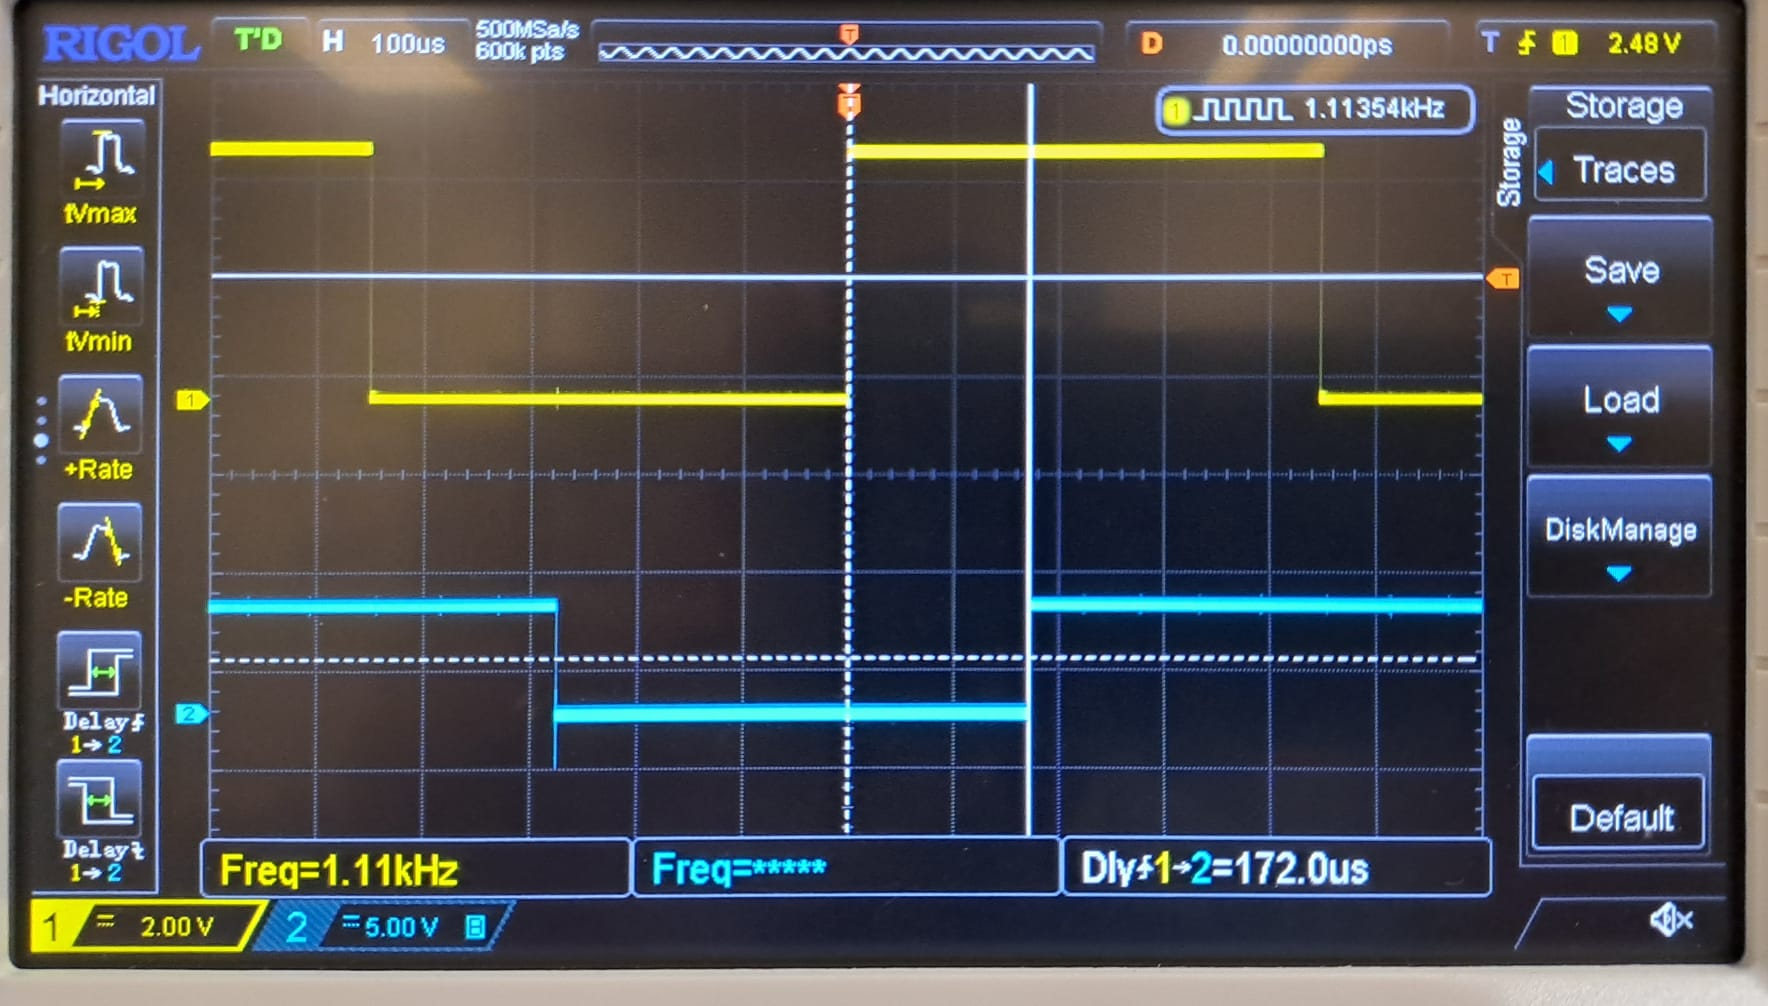
\includegraphics[width=1\linewidth]{img/1khz.jpeg}
      \caption{Circuito esquemático a montar: Amplificador sintonizado}%
      \label{fig:esque_ampl}
    \end{figure}
    
    \paragraph*{}
    Como de puede observar, se trata de un circuito con una etapa diferencia adaptada (puesto que no tenemos manera de invertir la señal e introducir 
    exactamente las tensiones positivas y negativas en ambos lados del diferencial) que junto con las bobinas y condensador que unen las dos etapas 
    se obtiene un amplificador de tensión sintonizado. La tensión de salida será la resta del lado izquierdo y derecho del condensador $C_1$, la cual 
    podremos medir con las herramientas que nos presta el osciloscopio. 
    
  

\vspace*{1.0cm}

    \begin{table}[H]
      \begin{center}
          \begin{tabular}{| c | c | c | c |}
              \hline
              \rowcolor{black}
              \textcolor{white}{$F_{ref}$ (kHz)} & \textcolor{white}{$F_{VCO}$ (kHz)} & \textcolor{white}{$\Delta \phi$ ($\mu$ s)} & \textcolor{white}{$V_{VCO}$ (V)}\\ \hline
              1.24 & 15.6 & 172 &  2.12\\ \hline
              1.511 & 23.8 & 144 &  2.35\\ \hline
              1.911 & 29.4 & 124 &  2.61\\ \hline
              2.378 & 35.7 & 114 & 2.91\\ \hline
              2.901 & 41.7 & 102 &  3.27\\ \hline
              3.142 & 47.2 & 100 & 3.44\\ 
              \hline 
          \end{tabular}
          \caption{Tabla de resultados reales de la práctica}
          \label{tab:resul_r}
      \end{center}
    \end{table}

  \paragraph*{}
    De la tabla anterior, se puede recalcar que en el polo de funcionamiento del amplificador ($f_0 = 11 kHz$) es cuando el amplificador tiene un mejor desempeño aplicando una ganancia de 
    aproximadamente 30. Si nos vamos alejando poco a poco de dicho polo, vemos como la ganancia cae rápidamente, por lo que podemos intuir que su comportamiento en el dominio de Laplace será 
    un filtro paso banda de segundo orden. 

    \paragraph*{}
    Para ver ésto más en profundidad, en el apartado siguiente se dibujará el diagrama de bode del amplificador y se comparará con su diagrama ideal. 

  \section{Apartado 3}

    \paragraph*{}
    En este apartado se dibujará el diagrama de bode del amplificador sintonizado construido a partir de los valores obtenidos y además se comparará con su función ideal. 

    \paragraph*{}
    El diagrama de bode obtenido del circuito construido es el siguiente: 
   
    \begin{figure}[H]
      \centering
      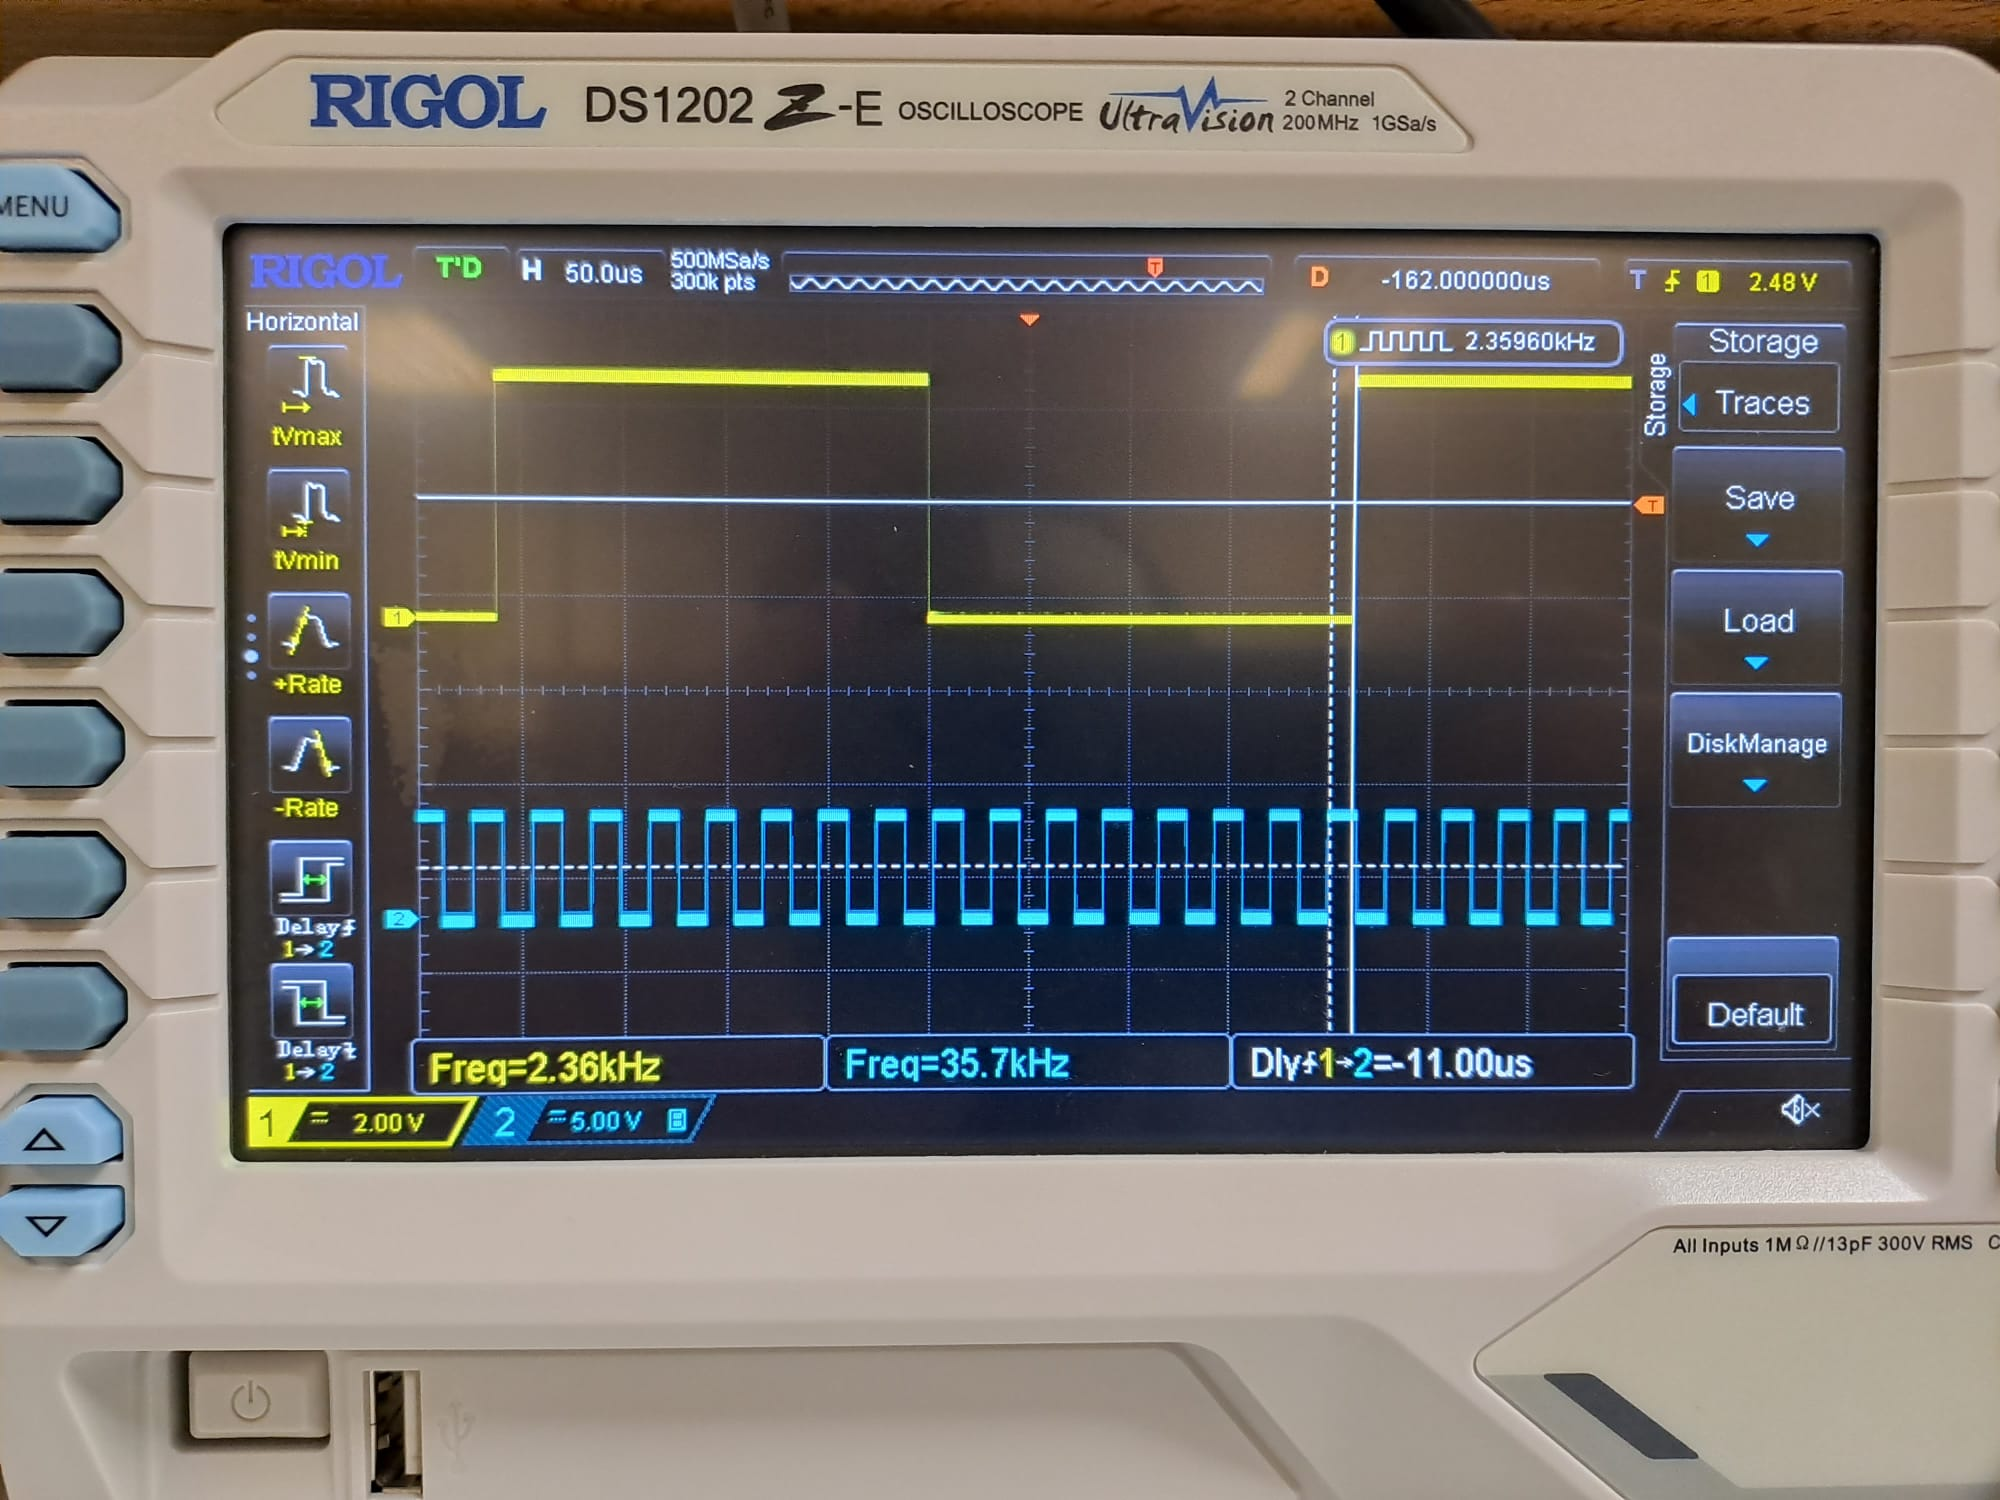
\includegraphics[width=1\linewidth]{img/2khz.jpeg}
      \caption{Diagrama de bode del circuito construido}%
      \label{fig:bode_real}
    \end{figure}
    
    \paragraph*{}
    Como se puede observar, tenemos un pico de ganancia máxima en la frecuencia del polo de funcionamiento del amplificador, en 11 kHz, alrededor de él la ganancia aplicada 
    recae rápidamente. 

    \paragraph*{}
    Un diagrama de bode de un filtro paso banda de segundo orden ideal, sería el siguiente: 

    \begin{figure}[H]
      \centering
      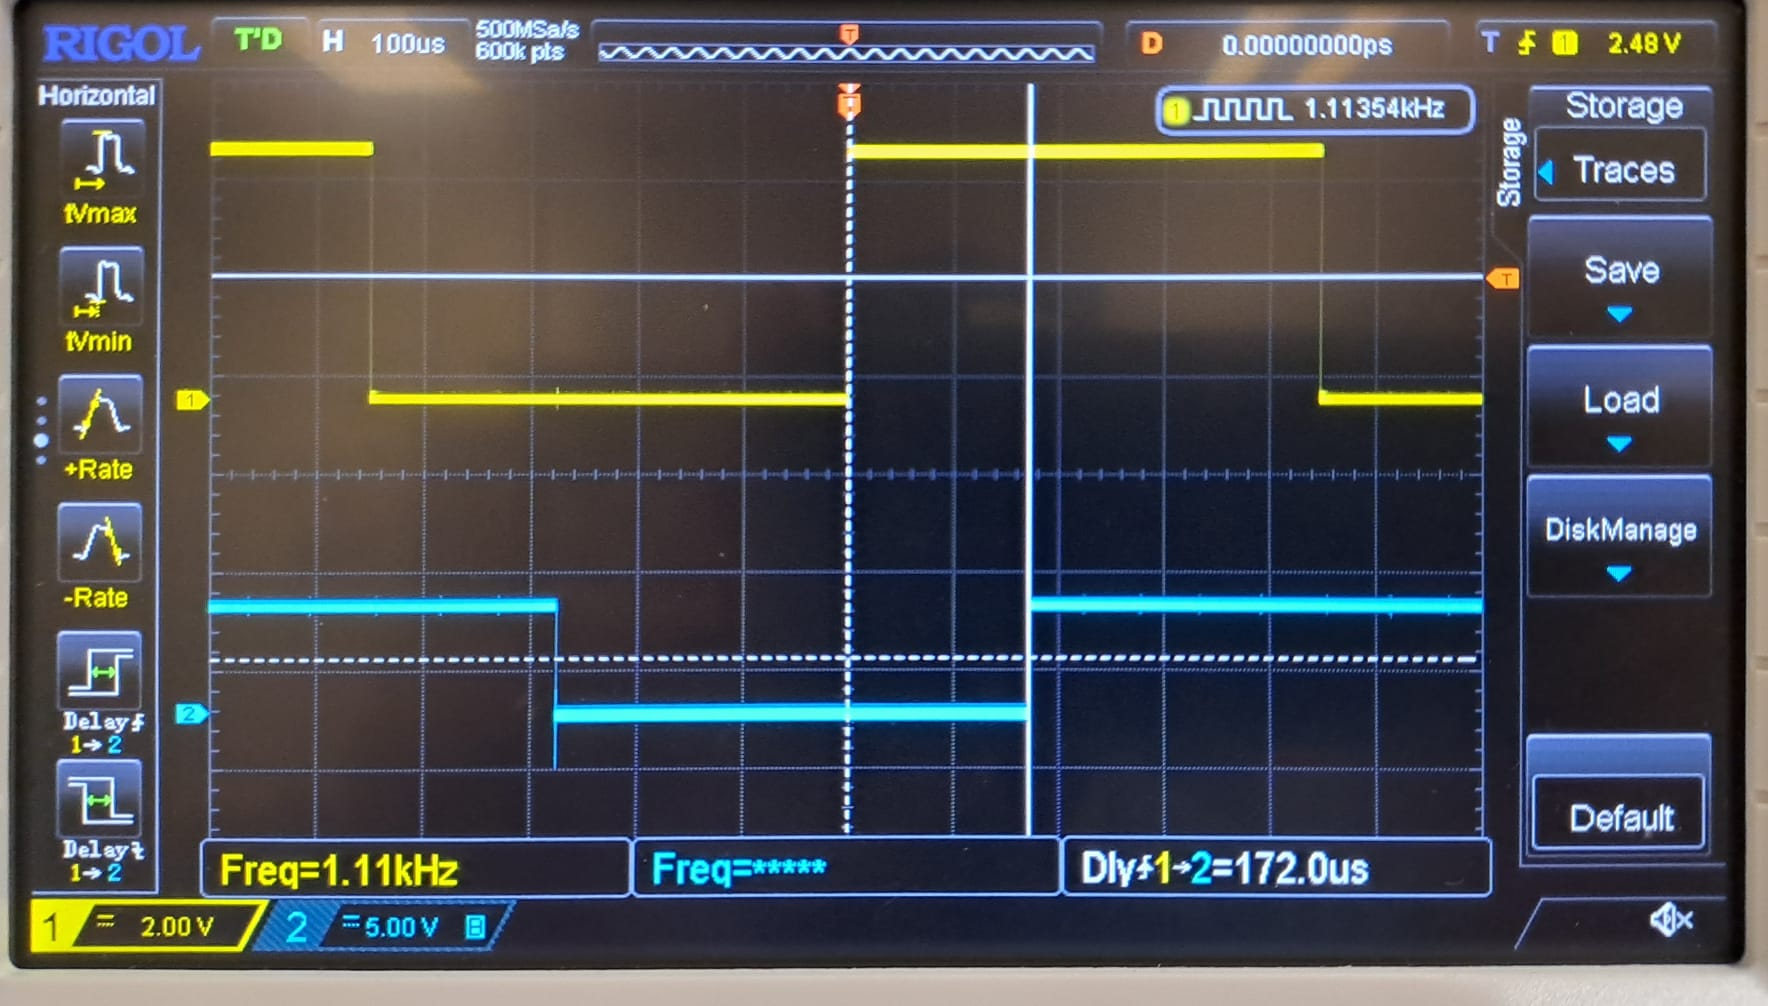
\includegraphics[width=1\linewidth]{img/1khz.jpeg}
      \caption{Diagrama de bode un filtro paso banda ideal de segundo orden}%
      \label{fig:bode_ideal}
    \end{figure}
    
    \paragraph*{}
    Podemos observar que el comportamiento en cuanto a la magnitud del filtro y el diagrama de bode real del amplificador son muy similares, por lo que concluimos que el funcionamiento 
    del amplificador es el adecuado teniendo en cuenta los datos medidos. 

    \paragraph*{}
    Cabe recalcar que para que los diagramas de bode reales e ideales mostrados sean más similares, es necesario obtener más valores de medida en saltos más pequeños en eje de frecuencias. 
    Por otro lado, el comportamiento de la fase en el diagrama de bode real no corresponde con la fase ideal debido a que para representar correctamente el comportamiento del amplificador 
    habría que calcular la función de transferencia en el dominio de Laplace y usar herramientas como Matlab para representarlo (de la misma manera como se calculo el diagrama de bode ideal
    con una función de transferencia genérica de un filtro paso banda ideal).

  \section{Apartado 4}

    \paragraph*{}
    La diferencia entre los resultados medidos en el laboratorio y los resultados de la simulación se debe principalmente a la resistencia parásita
    que aparece en las bobinas reales. Por tanto, para una mayor exactitud entre los resultados reales y los simulados, basta con añadir una resistencia en serie
    con dichas bobinas. %El valor de la resistencia parásita que se pudo medir en el laboratorio es $R_{L} = 28 \omega$.  
    
    \paragraph*{}
    Utilizando los valores de 11 kHz y con una tensión de entrada de 100 mV (valores con los que se obtiene la máxima ganancia en el circuito real), se puede medir 
    que el valor real es: $G_{R_{f0}} \approx 30$  mientras que el valor ideal según al simulación es: $G_{I{f0}} \approx 86$. Para obtener resultamos similares 
    a los reales en la simulación, colocamos una resistencia en serie con cada una de las bobinas y vamos variando su valor hasta obtener aquel que haga que la ganacia 
    ideal sea la misma o muy parecida que la real. 
    
    \begin{figure}[H]
      \centering
      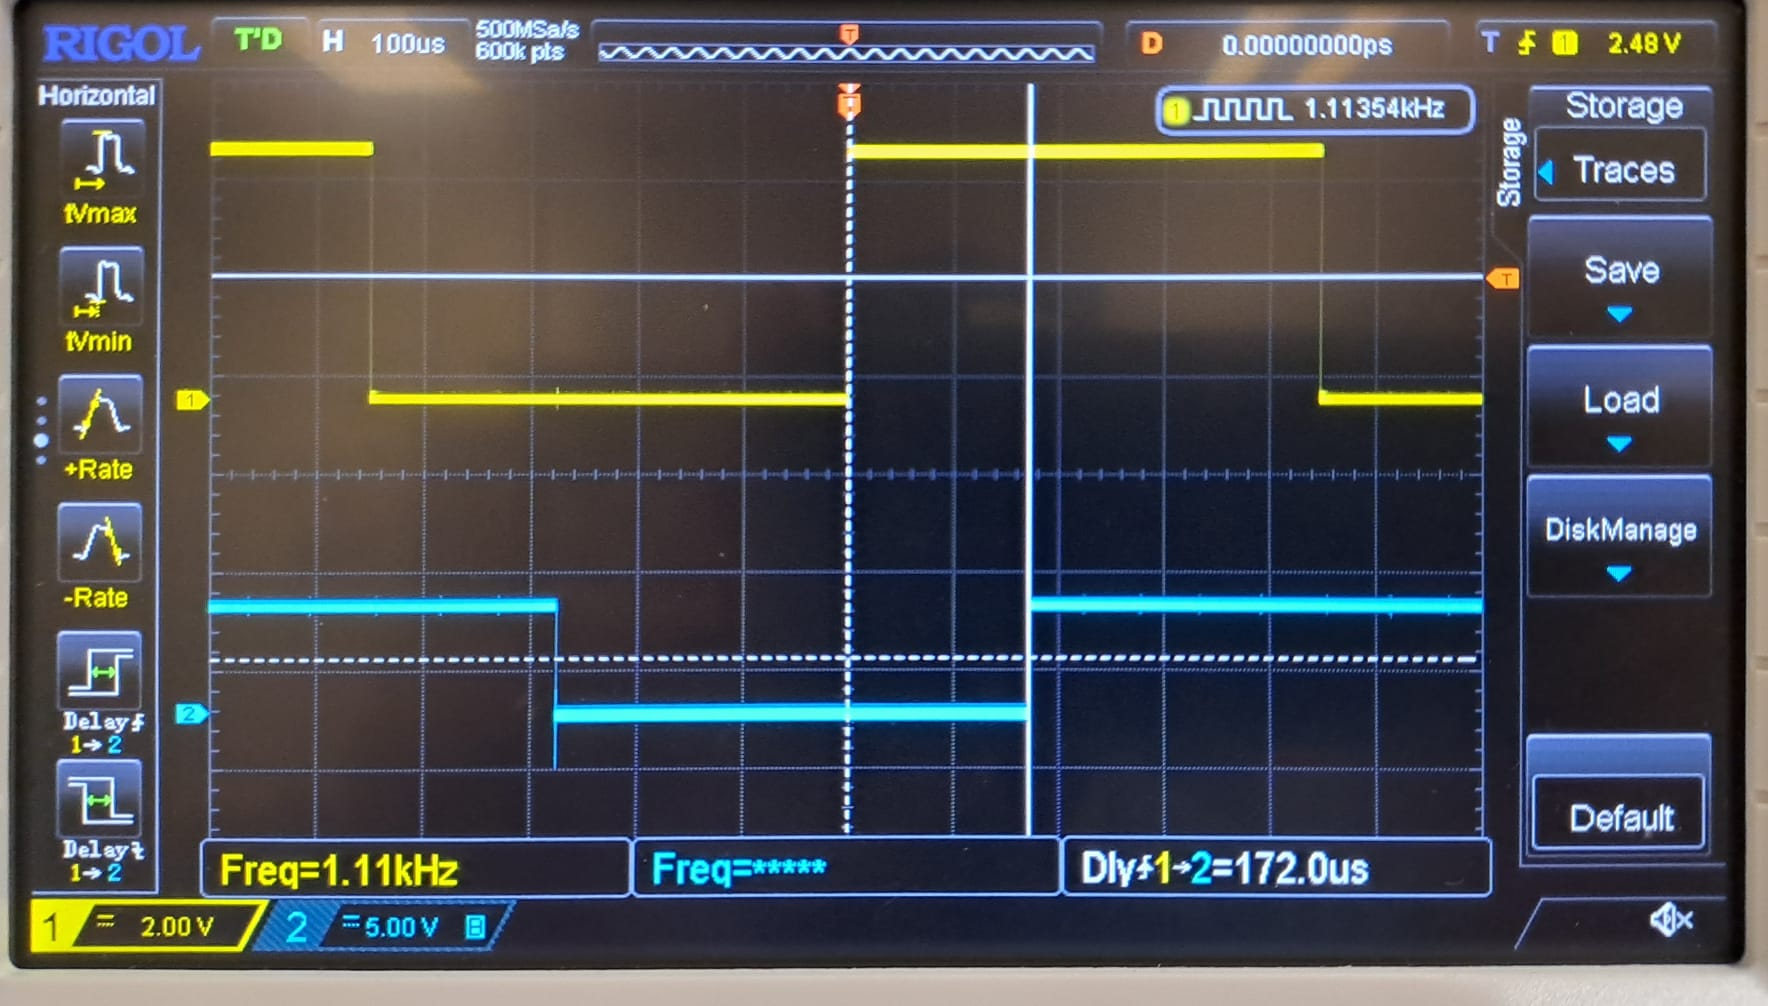
\includegraphics[width=1\linewidth]{img/1khz.jpeg}
      \caption{Simulación para la obtención de la resistencia parásita de las bobinas.}%
      \label{fig:res_bobina}
    \end{figure}
    
    \paragraph*{}
    Por lo tanto, obtenemos así una resistencia parásita en las bobinas de: $R_{L} \approx 10.7 \Omega$.


\end{document}